\documentclass{standalone}
\usepackage{tikz}
\usetikzlibrary{patterns, positioning}
\usepackage[sfdefault]{ClearSans} %% option 'sfdefault' activates Clear Sans as the default text font
\usepackage[T1]{fontenc}

\begin{document}
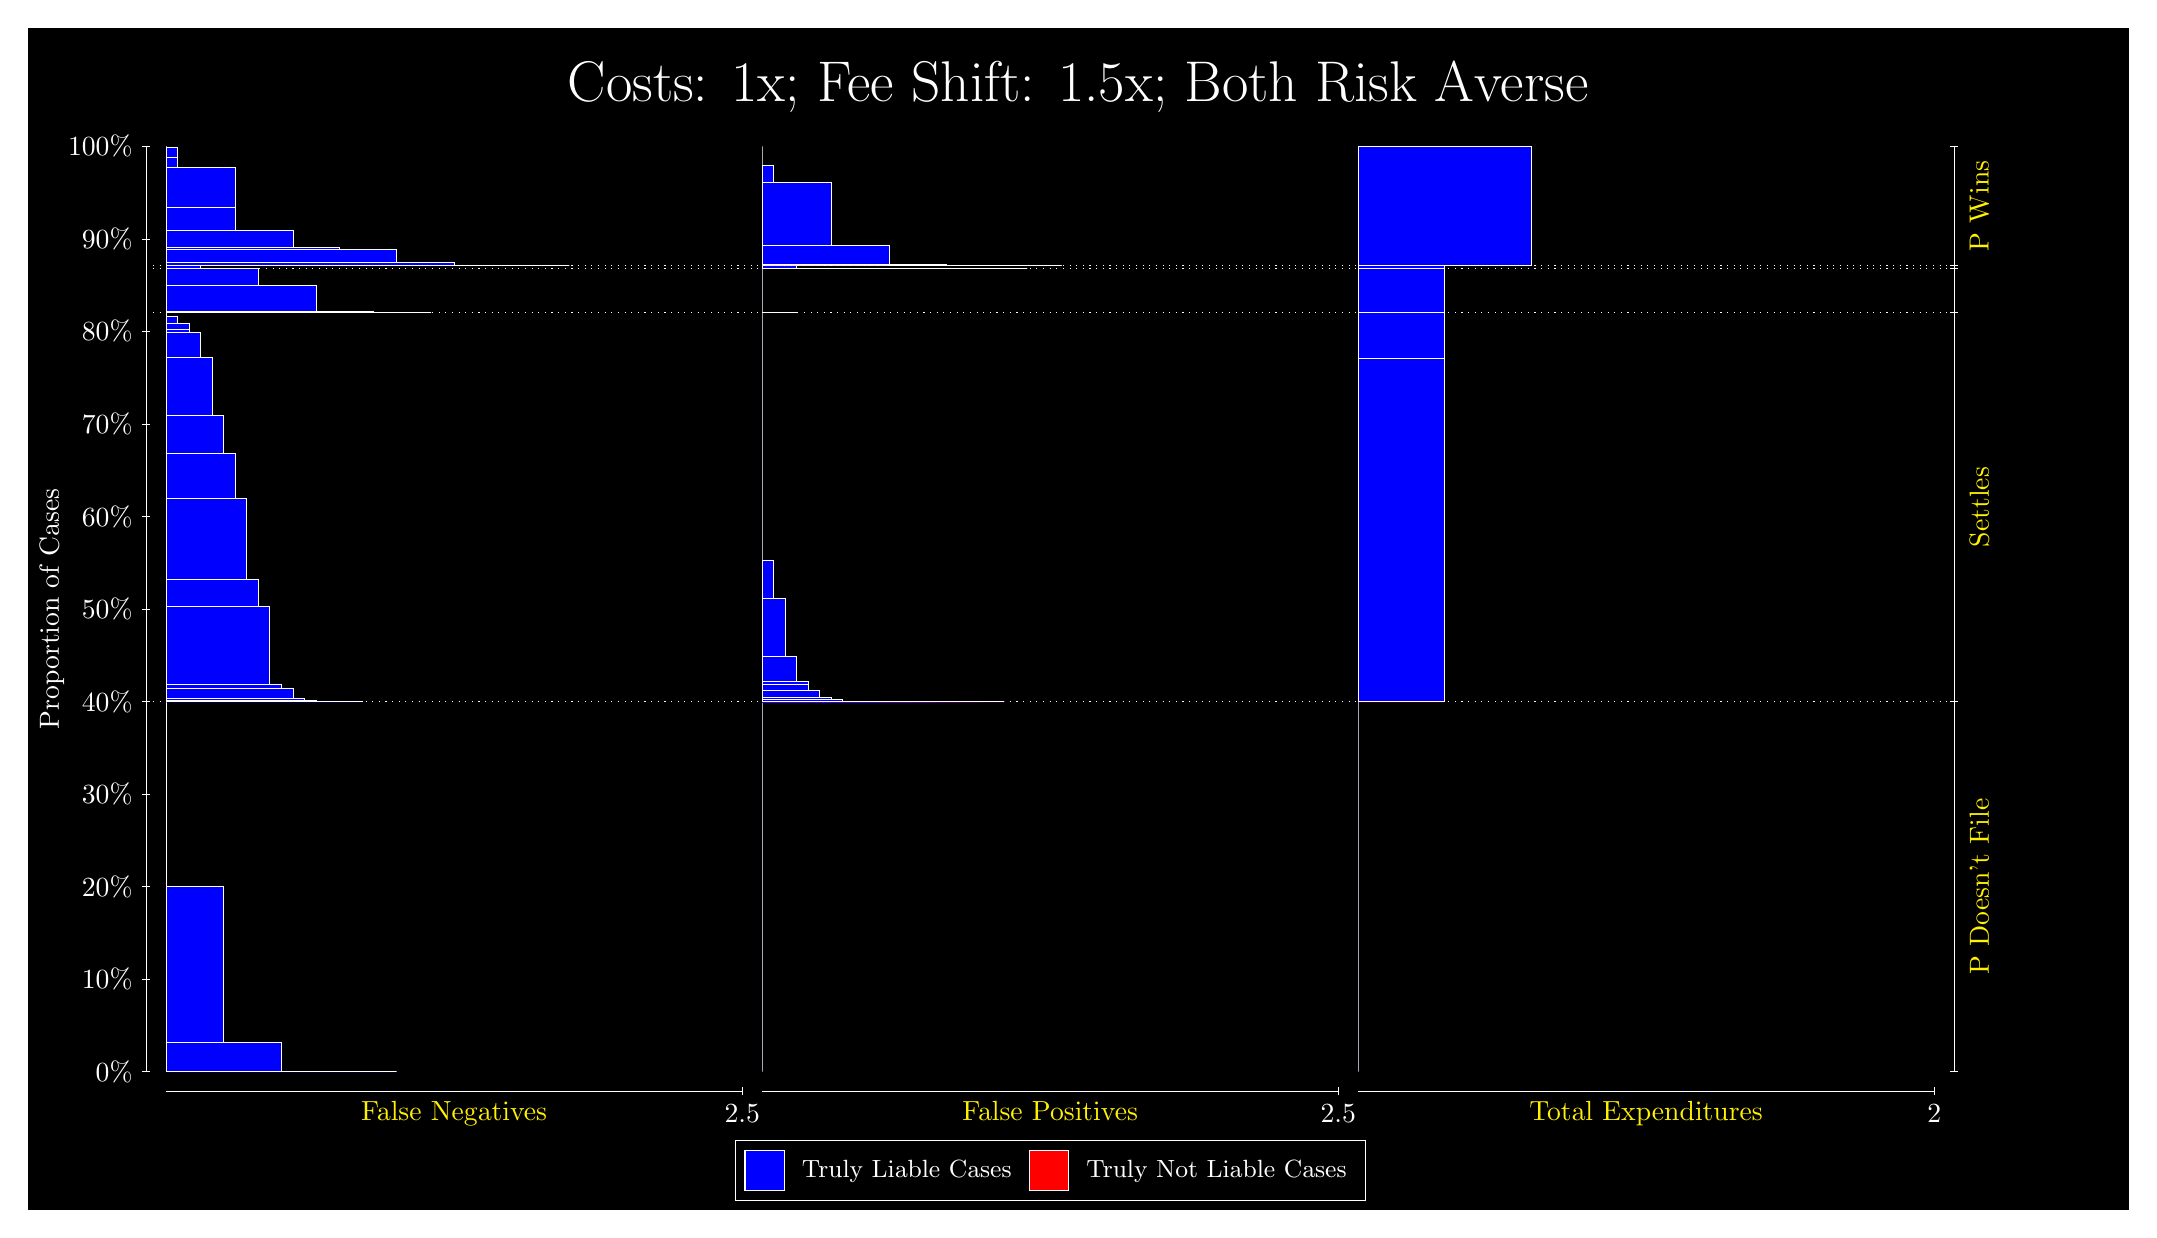
\begin{tikzpicture}
\draw[fill=black] (0,0) rectangle (26.667,15);
\draw[text=white] (0,13.5) rectangle (26.667,15) node[midway] {\huge Costs: 1x; Fee Shift: 1.5x; Both Risk Averse};
\draw[white, very thin] (1.5,1.75) -- (1.5,13.5);
\node[rotate=90, text=white, anchor=center] at (0.3, 7.625) {Proportion of Cases};
\draw[white, very thin] (1.45,1.75) -- (1.55,1.75);
\node[text=white, anchor=east] at (1.45, 1.75) {0\%};
\draw[white, very thin] (1.45,2.925) -- (1.55,2.925);
\node[text=white, anchor=east] at (1.45, 2.925) {10\%};
\draw[white, very thin] (1.45,4.1) -- (1.55,4.1);
\node[text=white, anchor=east] at (1.45, 4.1) {20\%};
\draw[white, very thin] (1.45,5.275) -- (1.55,5.275);
\node[text=white, anchor=east] at (1.45, 5.275) {30\%};
\draw[white, very thin] (1.45,6.45) -- (1.55,6.45);
\node[text=white, anchor=east] at (1.45, 6.45) {40\%};
\draw[white, very thin] (1.45,7.625) -- (1.55,7.625);
\node[text=white, anchor=east] at (1.45, 7.625) {50\%};
\draw[white, very thin] (1.45,8.8) -- (1.55,8.8);
\node[text=white, anchor=east] at (1.45, 8.8) {60\%};
\draw[white, very thin] (1.45,9.975) -- (1.55,9.975);
\node[text=white, anchor=east] at (1.45, 9.975) {70\%};
\draw[white, very thin] (1.45,11.15) -- (1.55,11.15);
\node[text=white, anchor=east] at (1.45, 11.15) {80\%};
\draw[white, very thin] (1.45,12.325) -- (1.55,12.325);
\node[text=white, anchor=east] at (1.45, 12.325) {90\%};
\draw[white, very thin] (1.45,13.5) -- (1.55,13.5);
\node[text=white, anchor=east] at (1.45, 13.5) {100\%};

\draw[white, very thin] (24.457,1.75) -- (24.457,13.5);
\draw[white, very thin] (24.407,1.75) -- (24.507,1.75);
\node[anchor=west] at (24.407, 1.75) {};
\draw[white, very thin] (24.407,6.4489) -- (24.507,6.4489);
\node[anchor=west] at (24.407, 6.4489) {};
\draw[white, very thin] (24.407,11.39) -- (24.507,11.39);
\node[anchor=west] at (24.407, 11.39) {};
\draw[white, very thin] (24.407,11.949) -- (24.507,11.949);
\node[anchor=west] at (24.407, 11.949) {};
\draw[white, very thin] (24.407,11.987) -- (24.507,11.987);
\node[anchor=west] at (24.407, 11.987) {};
\draw[white, very thin] (24.407,13.5) -- (24.507,13.5);
\node[anchor=west] at (24.407, 13.5) {};

\draw[white, very thin, fill=blue] (1.75,1.75) rectangle (4.6775,1.75);
\draw[white, very thin, fill=blue] (1.75,1.75) rectangle (3.9457,1.7532);
\draw[white, very thin, fill=blue] (1.75,1.7532) rectangle (3.2138,2.126);
\draw[white, very thin, fill=blue] (1.75,2.126) rectangle (2.4819,4.1027);
\draw[white, very thin, fill=red] (1.75,4.1027) rectangle (1.75,4.1027);
\draw[white, very thin, fill=blue] (1.75,4.1027) rectangle (1.75,6.4489);
\draw[white, very thin, fill=blue] (1.75,6.4489) rectangle (4.2384,6.449);
\draw[white, very thin, fill=blue] (1.75,6.449) rectangle (3.9457,6.4491);
\draw[white, very thin, fill=blue] (1.75,6.4491) rectangle (3.6529,6.4603);
\draw[white, very thin, fill=blue] (1.75,6.4603) rectangle (3.5065,6.4867);
\draw[white, very thin, fill=blue] (1.75,6.4867) rectangle (3.3602,6.614);
\draw[white, very thin, fill=blue] (1.75,6.614) rectangle (3.2138,6.6642);
\draw[white, very thin, fill=blue] (1.75,6.6642) rectangle (3.0674,7.6629);
\draw[white, very thin, fill=blue] (1.75,7.6629) rectangle (2.921,7.9968);
\draw[white, very thin, fill=blue] (1.75,7.9968) rectangle (2.7746,9.0347);
\draw[white, very thin, fill=blue] (1.75,9.0347) rectangle (2.6283,9.6023);
\draw[white, very thin, fill=blue] (1.75,9.6023) rectangle (2.4819,10.081);
\draw[white, very thin, fill=blue] (1.75,10.081) rectangle (2.3355,10.819);
\draw[white, very thin, fill=blue] (1.75,10.819) rectangle (2.1891,11.134);
\draw[white, very thin, fill=blue] (1.75,11.134) rectangle (2.0428,11.177);
\draw[white, very thin, fill=blue] (1.75,11.177) rectangle (2.0428,11.25);
\draw[white, very thin, fill=blue] (1.75,11.25) rectangle (1.8964,11.338);
\draw[white, very thin, fill=red] (1.75,11.338) rectangle (1.75,11.338);
\draw[white, very thin, fill=blue] (1.75,11.338) rectangle (1.75,11.39);
\draw[white, very thin, fill=blue] (1.75,11.39) rectangle (5.1167,11.39);
\draw[white, very thin, fill=blue] (1.75,11.39) rectangle (4.3848,11.4);
\draw[white, very thin, fill=blue] (1.75,11.4) rectangle (3.6529,11.731);
\draw[white, very thin, fill=blue] (1.75,11.731) rectangle (2.921,11.947);
\draw[white, very thin, fill=blue] (1.75,11.947) rectangle (2.1891,11.949);
\draw[white, very thin, fill=red] (1.75,11.949) rectangle (1.75,11.949);
\draw[white, very thin, fill=blue] (1.75,11.949) rectangle (2.1891,11.983);
\draw[white, very thin, fill=red] (1.75,11.983) rectangle (1.75,11.983);
\draw[white, very thin, fill=blue] (1.75,11.983) rectangle (1.75,11.987);
\draw[white, very thin, fill=blue] (1.75,11.987) rectangle (6.8732,11.987);
\draw[white, very thin, fill=blue] (1.75,11.987) rectangle (6.1413,11.988);
\draw[white, very thin, fill=blue] (1.75,11.988) rectangle (5.4094,12.023);
\draw[white, very thin, fill=blue] (1.75,12.023) rectangle (4.8239,12.023);
\draw[white, very thin, fill=blue] (1.75,12.023) rectangle (4.6775,12.193);
\draw[white, very thin, fill=blue] (1.75,12.193) rectangle (4.092,12.193);
\draw[white, very thin, fill=blue] (1.75,12.193) rectangle (3.9457,12.223);
\draw[white, very thin, fill=blue] (1.75,12.223) rectangle (3.3602,12.438);
\draw[white, very thin, fill=blue] (1.75,12.438) rectangle (3.2138,12.438);
\draw[white, very thin, fill=blue] (1.75,12.438) rectangle (2.6283,12.732);
\draw[white, very thin, fill=blue] (1.75,12.732) rectangle (2.6283,13.239);
\draw[white, very thin, fill=blue] (1.75,13.239) rectangle (2.4819,13.239);
\draw[white, very thin, fill=blue] (1.75,13.239) rectangle (1.8964,13.365);
\draw[white, very thin, fill=blue] (1.75,13.365) rectangle (1.8964,13.488);
\draw[white, very thin, fill=red] (1.75,13.488) rectangle (1.75,13.488);
\draw[white, very thin, fill=blue] (1.75,13.488) rectangle (1.75,13.5);
\draw[white, very thin, fill=red] (9.3189,1.75) rectangle (9.3189,1.75);
\draw[white, very thin, fill=blue] (9.3189,1.75) rectangle (9.3189,6.4489);
\draw[white, very thin, fill=red] (9.3189,6.4489) rectangle (12.393,6.4489);
\draw[white, very thin, fill=blue] (9.3189,6.4489) rectangle (12.393,6.4489);
\draw[white, very thin, fill=red] (9.3189,6.4489) rectangle (12.1,6.4489);
\draw[white, very thin, fill=blue] (9.3189,6.4489) rectangle (12.1,6.4489);
\draw[white, very thin, fill=red] (9.3189,6.4489) rectangle (11.807,6.4489);
\draw[white, very thin, fill=blue] (9.3189,6.4489) rectangle (11.807,6.4489);
\draw[white, very thin, fill=blue] (9.3189,6.4489) rectangle (11.661,6.4489);
\draw[white, very thin, fill=red] (9.3189,6.4489) rectangle (11.515,6.4489);
\draw[white, very thin, fill=blue] (9.3189,6.4489) rectangle (11.515,6.4489);
\draw[white, very thin, fill=blue] (9.3189,6.4489) rectangle (11.368,6.4489);
\draw[white, very thin, fill=red] (9.3189,6.4489) rectangle (11.222,6.4489);
\draw[white, very thin, fill=blue] (9.3189,6.4489) rectangle (11.222,6.4489);
\draw[white, very thin, fill=blue] (9.3189,6.4489) rectangle (11.075,6.4489);
\draw[white, very thin, fill=red] (9.3189,6.4489) rectangle (10.929,6.4489);
\draw[white, very thin, fill=blue] (9.3189,6.4489) rectangle (10.929,6.4489);
\draw[white, very thin, fill=blue] (9.3189,6.4489) rectangle (10.783,6.4491);
\draw[white, very thin, fill=blue] (9.3189,6.4491) rectangle (10.636,6.4492);
\draw[white, very thin, fill=red] (9.3189,6.4492) rectangle (10.636,6.4492);
\draw[white, very thin, fill=blue] (9.3189,6.4492) rectangle (10.636,6.4492);
\draw[white, very thin, fill=blue] (9.3189,6.4492) rectangle (10.49,6.456);
\draw[white, very thin, fill=blue] (9.3189,6.456) rectangle (10.344,6.4805);
\draw[white, very thin, fill=blue] (9.3189,6.4805) rectangle (10.197,6.5008);
\draw[white, very thin, fill=blue] (9.3189,6.5008) rectangle (10.051,6.5893);
\draw[white, very thin, fill=blue] (9.3189,6.5893) rectangle (9.9044,6.6625);
\draw[white, very thin, fill=blue] (9.3189,6.6625) rectangle (9.9044,6.7055);
\draw[white, very thin, fill=blue] (9.3189,6.7055) rectangle (9.758,7.02);
\draw[white, very thin, fill=blue] (9.3189,7.02) rectangle (9.6116,7.7588);
\draw[white, very thin, fill=blue] (9.3189,7.7588) rectangle (9.4652,8.237);
\draw[white, very thin, fill=blue] (9.3189,8.237) rectangle (9.3189,11.39);
\draw[white, very thin, fill=red] (9.3189,11.39) rectangle (9.758,11.39);
\draw[white, very thin, fill=blue] (9.3189,11.39) rectangle (9.758,11.393);
\draw[white, very thin, fill=blue] (9.3189,11.393) rectangle (9.3189,11.949);
\draw[white, very thin, fill=red] (9.3189,11.949) rectangle (12.686,11.949);
\draw[white, very thin, fill=blue] (9.3189,11.949) rectangle (12.686,11.949);
\draw[white, very thin, fill=blue] (9.3189,11.949) rectangle (11.954,11.949);
\draw[white, very thin, fill=blue] (9.3189,11.949) rectangle (11.222,11.949);
\draw[white, very thin, fill=blue] (9.3189,11.949) rectangle (10.49,11.954);
\draw[white, very thin, fill=blue] (9.3189,11.954) rectangle (9.758,11.987);
\draw[white, very thin, fill=red] (9.3189,11.987) rectangle (13.125,11.987);
\draw[white, very thin, fill=blue] (9.3189,11.987) rectangle (13.125,11.987);
\draw[white, very thin, fill=red] (9.3189,11.987) rectangle (12.393,11.987);
\draw[white, very thin, fill=blue] (9.3189,11.987) rectangle (12.393,11.988);
\draw[white, very thin, fill=red] (9.3189,11.988) rectangle (11.661,11.988);
\draw[white, very thin, fill=blue] (9.3189,11.988) rectangle (11.661,11.999);
\draw[white, very thin, fill=red] (9.3189,11.999) rectangle (10.929,11.999);
\draw[white, very thin, fill=blue] (9.3189,11.999) rectangle (10.929,12.249);
\draw[white, very thin, fill=red] (9.3189,12.249) rectangle (10.344,12.249);
\draw[white, very thin, fill=blue] (9.3189,12.249) rectangle (10.344,12.249);
\draw[white, very thin, fill=blue] (9.3189,12.249) rectangle (10.197,13.049);
\draw[white, very thin, fill=red] (9.3189,13.049) rectangle (9.6116,13.049);
\draw[white, very thin, fill=blue] (9.3189,13.049) rectangle (9.6116,13.049);
\draw[white, very thin, fill=blue] (9.3189,13.049) rectangle (9.4652,13.265);
\draw[white, very thin, fill=red] (9.3189,13.265) rectangle (9.3189,13.265);
\draw[white, very thin, fill=blue] (9.3189,13.265) rectangle (9.3189,13.5);
\draw[white, very thin, fill=red] (16.888,1.75) rectangle (16.888,1.75);
\draw[white, very thin, fill=blue] (16.888,1.75) rectangle (16.888,6.4489);
\draw[white, very thin, fill=red] (16.888,6.4489) rectangle (17.986,6.4489);
\draw[white, very thin, fill=blue] (16.888,6.4489) rectangle (17.986,10.813);
\draw[white, very thin, fill=red] (16.888,10.813) rectangle (17.986,10.813);
\draw[white, very thin, fill=blue] (16.888,10.813) rectangle (17.986,11.39);
\draw[white, very thin, fill=red] (16.888,11.39) rectangle (17.986,11.39);
\draw[white, very thin, fill=blue] (16.888,11.39) rectangle (17.986,11.949);
\draw[white, very thin, fill=red] (16.888,11.949) rectangle (17.986,11.949);
\draw[white, very thin, fill=blue] (16.888,11.949) rectangle (17.986,11.987);
\draw[white, very thin, fill=red] (16.888,11.987) rectangle (19.083,11.987);
\draw[white, very thin, fill=blue] (16.888,11.987) rectangle (19.083,13.5);
\draw[white, dotted] (1.5,6.4489) -- (24.457,6.4489);
\draw[white, dotted] (1.5,11.39) -- (24.457,11.39);
\draw[white, dotted] (1.5,11.949) -- (24.457,11.949);
\draw[white, dotted] (1.5,11.987) -- (24.457,11.987);
\draw[white, very thin] (1.75,1.5) -- (9.0689,1.5);
\node[text=yellow, anchor=north] at (5.4094, 1.5) {False Negatives};
\draw[white, very thin] (9.0689,1.45) -- (9.0689,1.55);
\node[text=white, anchor=north] at (9.0689, 1.45) {2.5};

\draw[white, very thin] (9.3189,1.5) -- (16.638,1.5);
\node[text=yellow, anchor=north] at (12.978, 1.5) {False Positives};
\draw[white, very thin] (16.638,1.45) -- (16.638,1.55);
\node[text=white, anchor=north] at (16.638, 1.45) {2.5};

\draw[white, very thin] (16.888,1.5) -- (24.207,1.5);
\node[text=yellow, anchor=north] at (20.547, 1.5) {Total Expenditures};
\draw[white, very thin] (24.207,1.45) -- (24.207,1.55);
\node[text=white, anchor=north] at (24.207, 1.45) {2};

\node[text=yellow, centered, rotate=90] at (24.777, 4.0995) {P Doesn't File};
\node[text=yellow, centered, rotate=90] at (24.777, 8.9196) {Settles};


\node[text=yellow, centered, rotate=90] at (24.777, 12.744) {P Wins};

\draw (12.978300999999998,1.5) node[draw=none] (baseCoordinate) {};
\begin{scope}[align=center]
        \matrix[scale=0.5, draw=white, below=0.5cm of baseCoordinate, nodes={draw}, column sep=0.1cm]{
            \node[rectangle, draw, minimum width=0.5cm, minimum height=0.5cm, fill=blue] {}; &
            \node[draw=none, font=\small, text=white] (B) {Truly Liable Cases}; &
            \node[rectangle, draw, minimum width=0.5cm, minimum height=0.5cm, fill=red] {}; &
            \node[draw=none, font=\small, text=white] (B) {Truly Not Liable Cases}; \\
            };
\end{scope}

\end{tikzpicture}
\end{document}